\section{Istanze di esempio}
In questo capitolo mostreremo le istanze prese per verificare la correttezza del codice e per misurare le prestazioni del programma. Tali misurazioni verranno presentate nel prossimo capitolo riguardante appunto le prestazioni.

Abbiamo preso in esame quattro istanze di cui tre tratte dalla specifica del progetto fornitaci mentre la quarta è una istanza progettata da noi. Le prime due istanze prese dalla specifica sono servite in particolare per verificare che il codice fosse corretto e ha aiutato la fase di debug nei momenti in cui il programma non aveva un comportamento atteso. La terza istanza e quella da noi creata sono servite invece per misurare le prestazioni, sia in termini temporali, quanto tempo richiedesse per compiere una determinata operazione, sia in termini spaziali, ovvero effettivamente di quanta memoria il programma necessiti per la risoluzione del proprio compito.

Qui sotto mostriamo brevemente la struttura delle reti di automi che formano le varie istanze. Queste sono le rappresentazioni visive delle istanze date in input al programma.

Da notare che durante la presentazione dei risultati per \textit{Diagnosi Relativa all’osservazione lineare} si intende il risultato uscente dall'analisi dello spazio osservabile mentre per \textit{Diagnosi Lineare sull’osservazione lineare} si intende il risultato dell'esecuzione dell'analisi del diagnosticatore.

\subsection{Istanza di Base}
\subsubsection{Rappresentazione grafica}
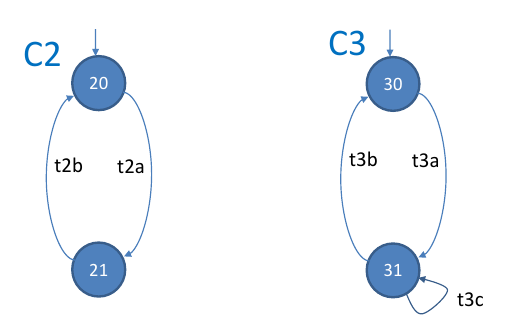
\includegraphics[width=\textwidth]{immagini/B1Rete.png}

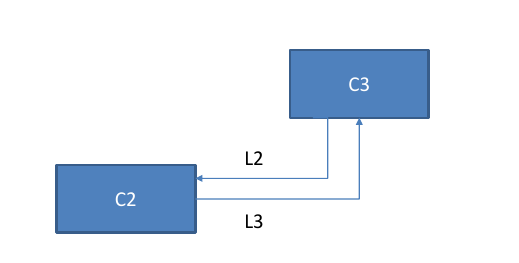
\includegraphics[width=\textwidth]{immagini/B1top.png}

\subsubsection{Etichette ed Eventi}

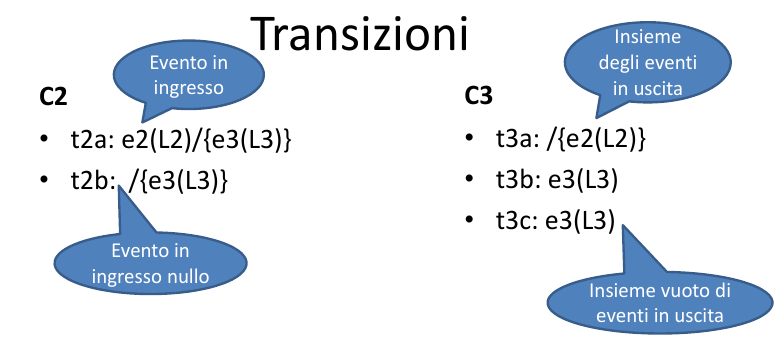
\includegraphics[width=\textwidth]{immagini/B1Trans.png}

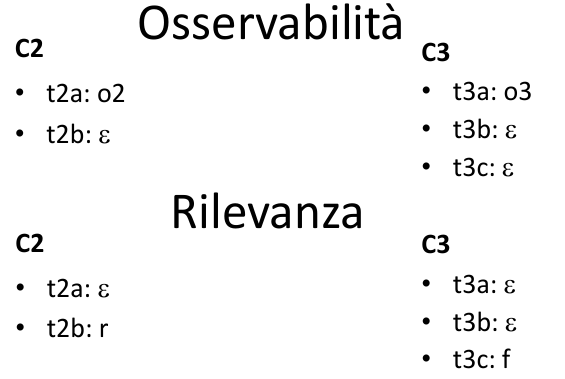
\includegraphics[width=\textwidth]{immagini/B1Oss.png}

\subsubsection{Risultati}
Diagnosi Relativa all'osservazione lineare $[o3, o2]$
\begin{itemize}
    \item  $fr\|frf\|\epsilon\|f$
\end{itemize}
Diagnosi Lineare sull'osservazione lineare $[o3, o2, o3, o2]$
\begin{itemize}
    \item $rf\|rffrf\|rffr\|rff$
    \item $fr\|frfrf\|frfr\|frf$
\end{itemize}

Il risultato completo dell'esecuzione è visionabile come immagine di seguito oltre che all'interno della reposity GitHub del progetto, nella cartella "Risultati Esempio" con il nome di "SummaryI1".

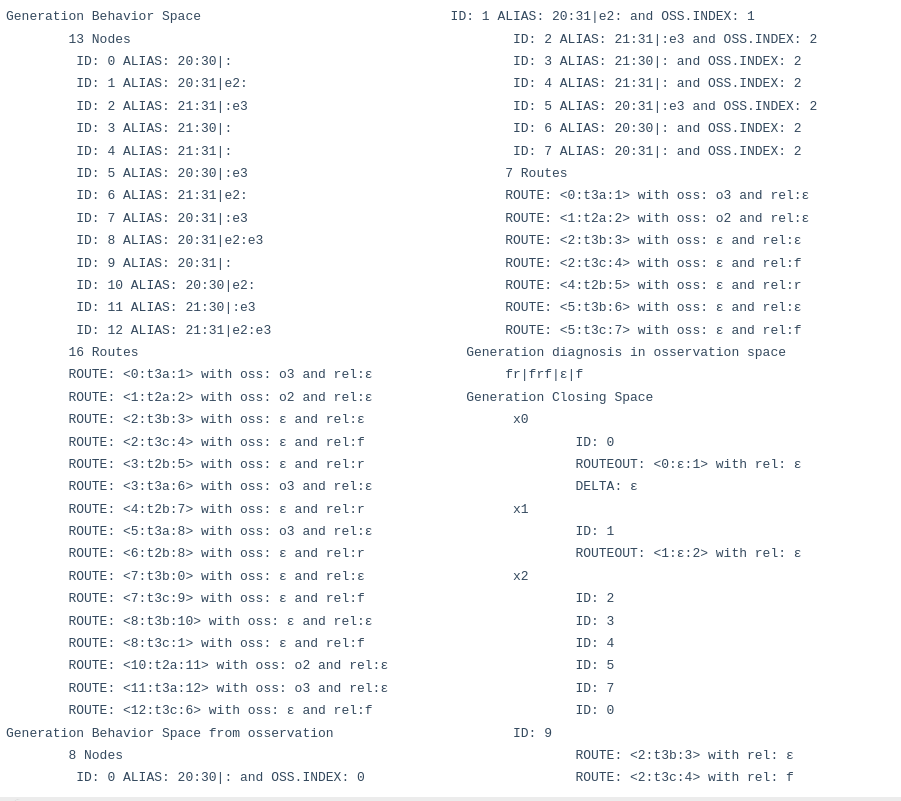
\includegraphics[width=\textwidth]{immagini/BI1.png}

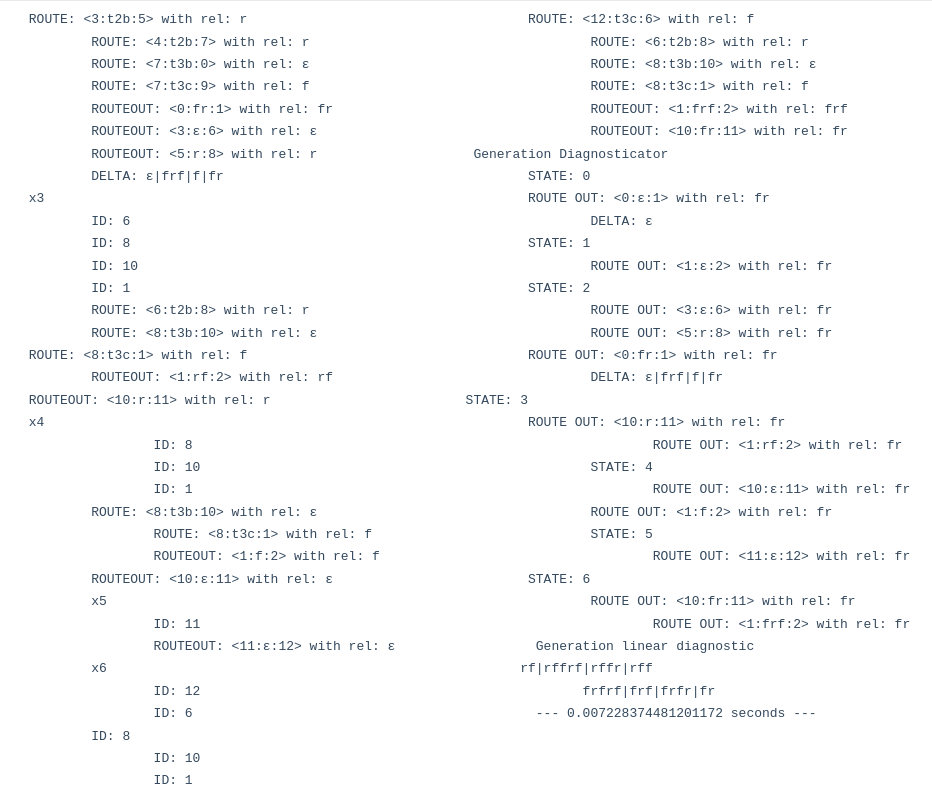
\includegraphics[width=\textwidth]{immagini/BI1_2.png}

\subsection{Istanza di Test}
\subsubsection{Rappresentazione grafica}
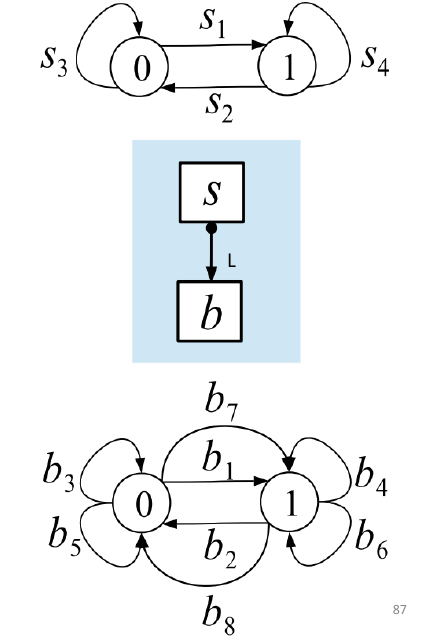
\includegraphics[width=\textwidth]{immagini/t1.png}

\subsubsection{Etichette ed Eventi}

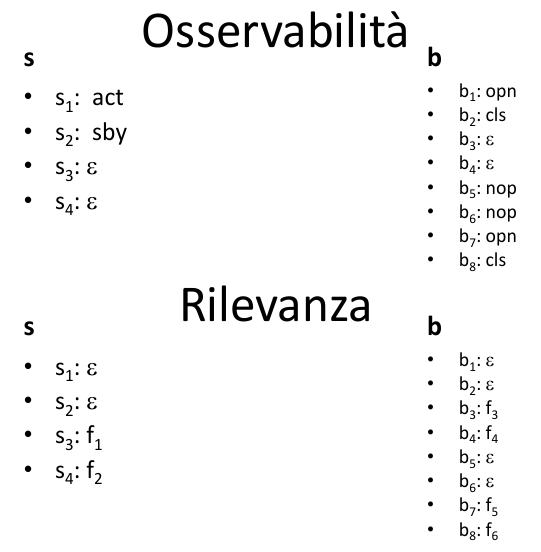
\includegraphics[width=\textwidth]{immagini/t1oss.png}

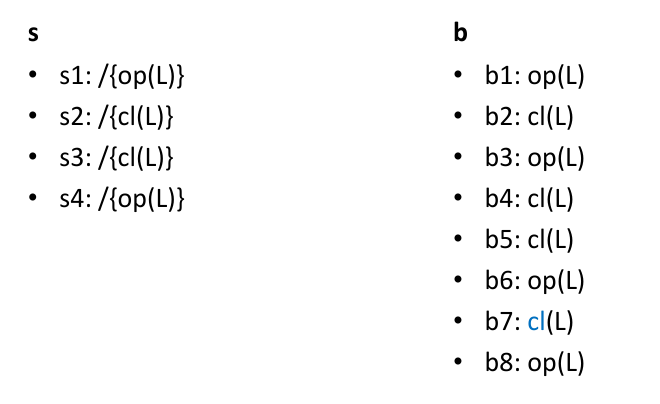
\includegraphics[width=\textwidth]{immagini/T1es.png}

\subsubsection{Risultati}
Diagnosi Relativa all'osservazione lineare $[act, sby, nop]$
\begin{itemize}
    \item  $(f3f2)^{*}f3$
\end{itemize}
Diagnosi Lineare sull'osservazione lineare $[act, sby, nop]$
\begin{itemize}
    \item $(f3f2)^{*}f3$
\end{itemize}

Il risultato completo dell'esecuzione è visionabile come immagine di seguito oltre che all'interno della reposity GitHub del progetto, nella cartella "Risultati Esempi" con il nome di "SummaryI2".

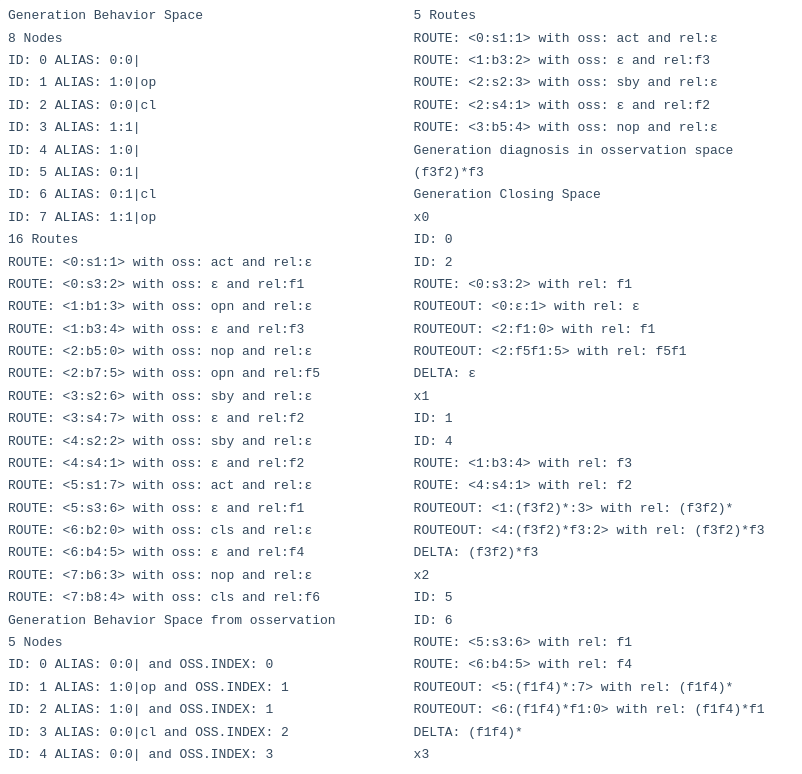
\includegraphics[width=\textwidth]{immagini/t1_1.png}

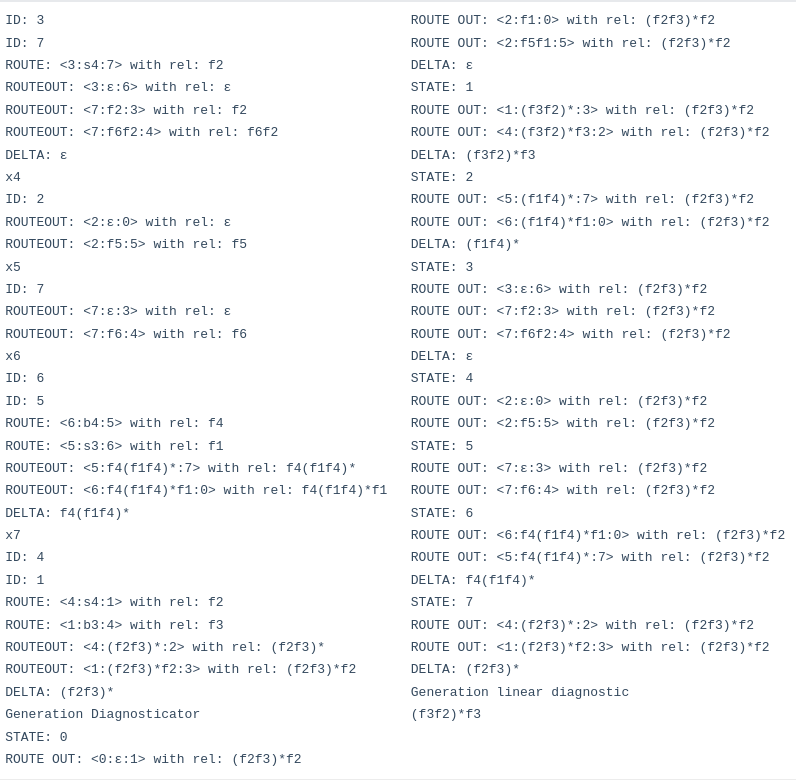
\includegraphics[width=\textwidth]{immagini/t1_2.png}

\subsection{Istanza di Benchmark}
\subsubsection{Rappresentazione grafica}
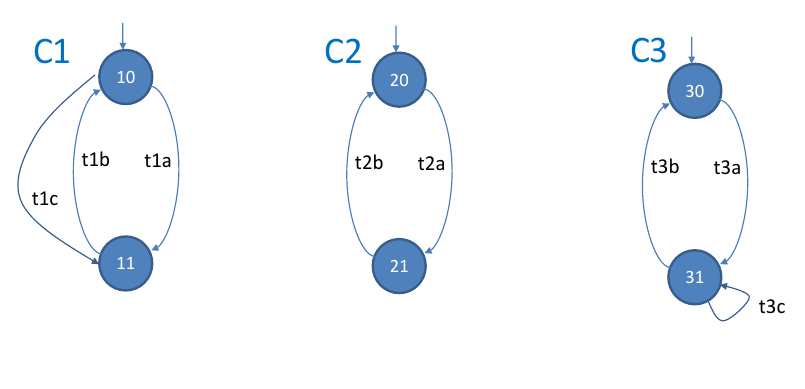
\includegraphics[width=\textwidth]{immagini/c1.png}

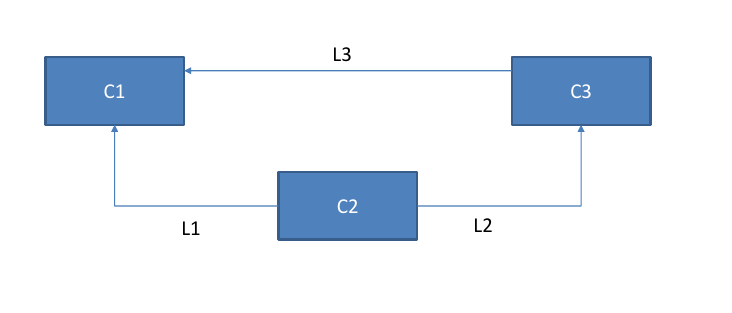
\includegraphics[width=\textwidth]{immagini/c2.png}

\subsubsection{Etichette ed Eventi}

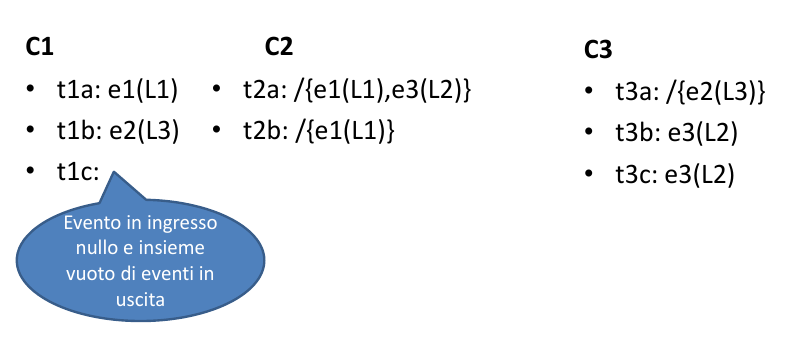
\includegraphics[width=\textwidth]{immagini/c3.png}

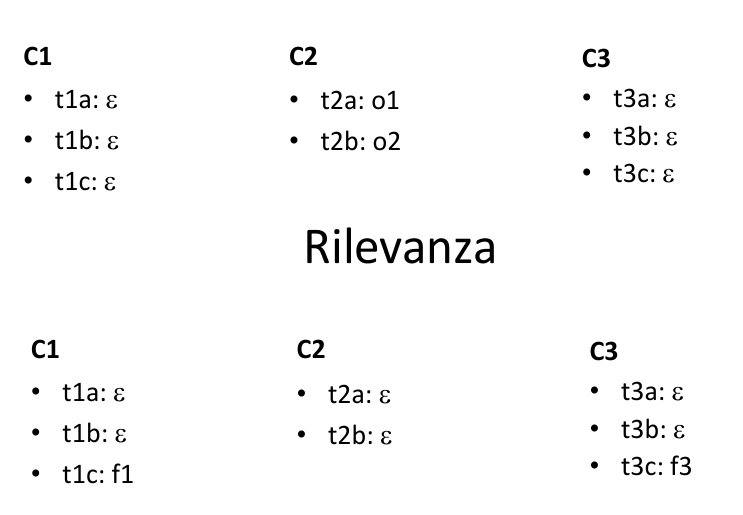
\includegraphics[width=\textwidth]{immagini/c4.png}

\subsubsection{Risultati}
Diagnosi Relativa all'osservazione lineare $[o1, o2]$
\begin{itemize}
    \item  $f3\|f1\|f1f1\|\epsilon$
\end{itemize}
Diagnosi Lineare sull'osservazione lineare $[o1, o2]$
\begin{itemize}
    \item $f3\|f1\|\epsilon$
    \item $f1\|\epsilon$
    \item $f1$
    \item $f3\|f1$
\end{itemize}

\subsection{Istanza creata da noi}
\subsubsection{Rappresentazione grafica}
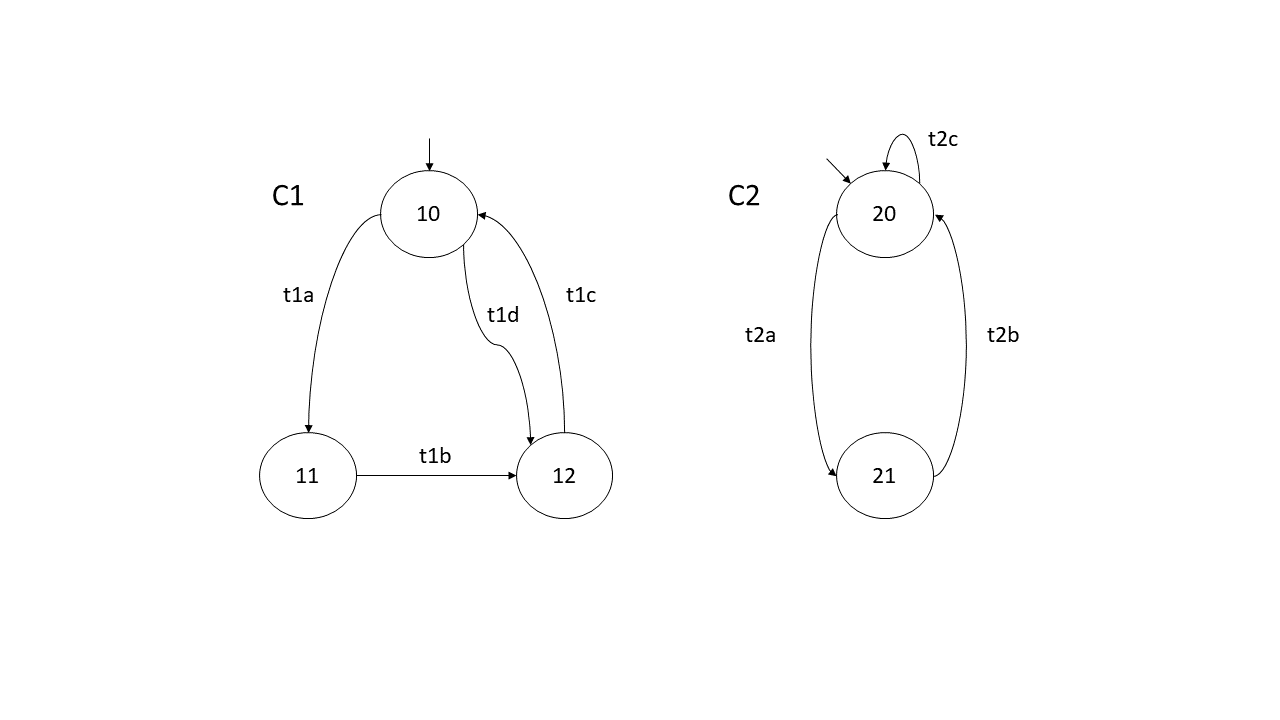
\includegraphics[width=\textwidth]{immagini/customFA.png}


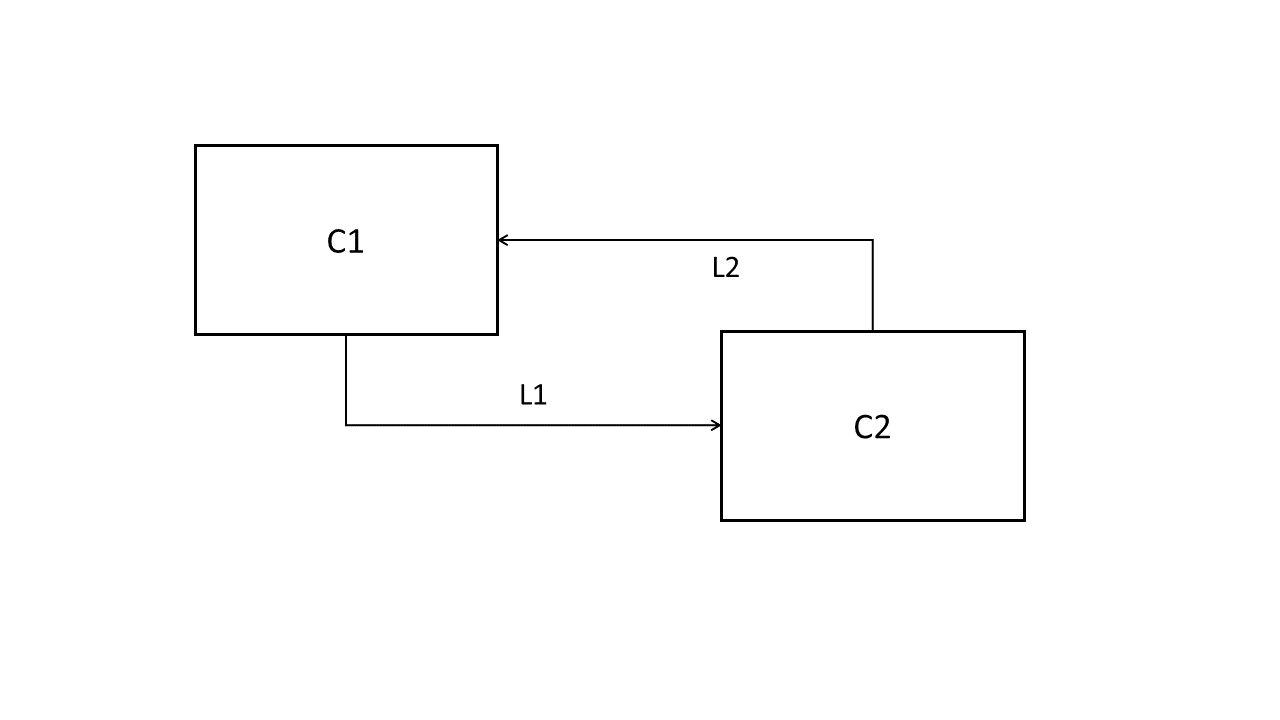
\includegraphics[width=\textwidth]{immagini/customNetFA.png}

\subsubsection{Etichette ed Eventi}
Etichette di osservazione:
\begin{itemize}
    \item t2b $\rightarrow$ \textbf{r}
    \item t2c $\rightarrow$ \textbf{f}
\end{itemize} 
Etichette di rilevanza:
\begin{itemize}
    \item t1a $\rightarrow$ \textbf{o1}
    \item t1d $\rightarrow$ \textbf{o2}
\end{itemize}

Eventi:
\begin{itemize}
    \item t1b $\rightarrow$ \textbf{\_\_:L1(e2)}
    \item t1d $\rightarrow$ \textbf{L2(e1):\_\_}
    \item t2b $\rightarrow$ \textbf{\_\_:L2(e1)}
    \item t2c $\rightarrow$ \textbf{L1(e2):\_\_}
\end{itemize}

\subsubsection{Risultati}
Diagnosi Relativa all'osservazione lineare $[o1, o2]$
\begin{itemize}
    \item  $rfr\|r\|rf\|fr\|frr\|\epsilon$
\end{itemize}
Diagnosi Lineare sull'osservazione lineare $[o1, o2, o1, o2]$
\begin{itemize}
    \item $rfrf\|frrf$
    \item $rfrf\|rrff$
    \item $rffr\|rfrf\|rrff$
\end{itemize}

\subsection{Dimensioni istanze}
Di seguito inseriamo alcune tabelle riassuntive che raccolgono le dimensioni dei vari spazi generati dal programma. Tali valori possono essere utili anche nel prossimo capitolo dove andiamo a commentare le prestazioni del software.

\begin{table}[h]
    \centering
    \begin{tabular}{ l | l l l l}
        & I1 & I2 & Icustom & \textbf{Ibenchmark}\\
        \hline
        \rowcolor{yellow} \emph{Nodi} & 13 & 8 & 23 & 41 \\
        \emph{Rotte}& 16 & 16 & 46 & 85 \\
        \hline
        \rowcolor{mygray} \textbf{Totale elementi} & 29 & 24 & 69 & 126 \\
        
    \end{tabular}
    \caption{Tabella relativa al numero di elementi generati dagli spazi comportamentali delle istanze presentate}
    \label{tab:tabella-behavior}
\end{table}

\begin{table}[h]
    \centering
    \begin{tabular}{ l | l l l l}
        & I1 & I2 & Icustom & \textbf{Ibenchmark}\\
        \hline
        \emph{Chiusure}  & 7 & 8 & 11 & 17\\
        \rowcolor{yellow} \emph{Nodi} & 22 & 14 & 136 & 177 \\
        \emph{Rotte} & 15 & 10 & 185 & 256 \\
        \emph{Rotte di output} & 12 & 18 & 88 & 64\\
        \hline
        \rowcolor{mygray} \textbf{Totale elementi} & 56 & 50 & 420 & 514 \\
        
    \end{tabular}
    \caption{Tabella relativa al numero di elementi generati dagli spazi delle chiusure delle istanze presentate}
    \label{tab:tabella-closures}
\end{table}
